\chapter{Industrial setting}
\label{chap:model}


\minitoc


%We start by defining what is this data and what ``interesting correlations'' means in our context.

Our contributions are integrated in the \datalyse project,
more precisely in the sub-project on business intelligence for the retail domain.
This part of the project involves 3 companies and our laboratory,
collaborating to find precise and relevant insights on customer behavior for marketing experts.
These companies are:
\begin{itemize}
	\item Intermarch\'e, that provides anonymized data and evaluates the  results,
	\item Business \& D\'ecision, assisting Intermarch\'e for data acquisition, and
	\item Eolas, that is hosting the system we present in this chapter.
\end{itemize}

Our own work aims at solving the challenges raised by the analysis of customer data
from a nation-wide retailer like Intermarch\'e.
To this end, we propose innovative algorithms and methods in the following chapters.
As a preliminary, in this chapter we describe the analytics workflow in which our contributions fit.


In Section~\ref{sec:pipeline:theirs} we give an overview of the data prepared by our partners:
customer files, product information and, chiefly, receipts.
Our complete analytics pipeline can be summarized as follows:

\begin{figure*}[h!]
	\centering
	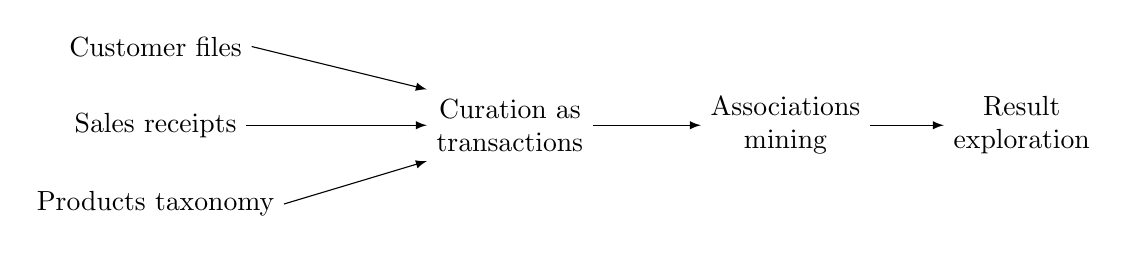
\begin{tikzpicture}[>=latex]
    \node (customer) at (-5,1) {Customer files};

    \node (receipts) at (-5,0) {Sales receipts};

    \node (taxonomy) at (-5,-1) {Products taxonomy};

    \node [align=center](transformation) at (-0.5,0) {Curation as\\transactions};
    \draw [->] (customer.east) -- (transformation.north west);
    \draw [->] (receipts.east) -- (transformation.west);
    \draw [->] (taxonomy.east) -- (transformation.south west);

    \node [align=center](mining) at (3,0) {Associations\\mining};
    \draw [->] (transformation.east) -- (mining.west);

    \node [align=center](exploration) at (6,0) {Result\\exploration};
    \draw [->] (mining.east) -- (exploration.west);
	\end{tikzpicture}
\end{figure*}


As we are considering millions of receipts generated by millions of customers,
each step requires specific systems to process this data reliably and in a reasonable amount of time.
We specify these in Section~\ref{sec:pipeline:ours},
and illustrate how itemsets can represent various patterns of user behavior
by defining 3 mining scenarios representative of marketing analysts' work.
% with excerpts from real data

%Therefore, although our contributions only concern the last steps of the process (mining and exploration),
%we also detail the curation step ({\em ie.} the construction of transactional datasets).
%This also allow us to describe the systems we have at hand,
%in particular for the mining step.

In order to validate the performance of our mining algorithm, \toppi,
we include two Web datasets (curated independently) in our collection.
We conclude in Section~\ref{sec:model:conc} by presenting all our datasets of interest,
and highlighting their common characteristics
that serve as a basis to our work.

%This also positions precisely our contributions and how they are integrated towards the production system.


Figure~\ref{fig:archoverview} gives a schematic representation of the system's components.
The first module, \textbf{acquisition and storage}, performs the classic data warehousing tasks.
The \textbf{curation} module is used to build transactions,
which are then processed by one of our \textbf{mining} programs.
Finally, the \textbf{exploitation} application allows the analyst to interactively explore results.

The complete data mining process relies on 5 steps:
\begin{enumerate}
	\item Sales records are produced locally at each store, and imported daily into
		Intermarch\'e's data center.
	\item Receipts are stored in a \textit{sales} table, where they can be
		joined with customer segments coming from the \textit{customers} table.
		The same database holds the \textit{taxonomy} table.
	\item The analyst selects one of our 3 analysis scenario,
		sets the required parameters (detailed in the corresponding chapters) and
		optionally defines ``targets'', which are items of interest.
		%(this is only relevant for \capa and \jlcm).
	The collection of transactions {\mf D} is generated accordingly.
	\item The required itemset mining algorithm is executed on {\mf D}.
	\item Resulting itemsets are converted to association rules
		and loaded in a relational database dedicated to the exploration application.
\end{enumerate}

\vfill
{
\newgeometry{top=1in, bottom=1.25in, left=0.75in, right=0.75in}
	\begin{figure}
		\begin{minipage}{\textwidth}
			\tikzset{
    rulesTable/.style={
        matrix of nodes,
        row sep=-\pgflinewidth,
        column sep=-\pgflinewidth,
        nodes={
            rectangle,
            draw=black,
            align=center
        },
        minimum height=1em,
        minimum width=1em,
        text width=1em,
        text depth=0.5ex,
        text height=1ex,
        nodes in empty cells,
        %%
        every even row/.style={
            nodes={fill=black!30}
        },
        row 1/.style={
            nodes={
                fill=black!60,
                text=white,
                font=\small\bfseries
            }
        }
    }
}
\tikzset{element/.style={rectangle,
        inner sep=0pt,
        minimum width=1mm,
        draw=black,
        top color=blue!20!white!20,
        bottom color=blue!70!white,
}}

\tikzstyle{doc}=[%
	draw,
	thick,
	align=center,
	color=black,
	shape=rectangle,
	minimum width=10mm,
	minimum height=18.2mm,
	inner sep=2ex
]

\tikzset{
	comp/.style = {
		minimum width  = 3.5cm,
		minimum height = 2cm,
		text width     = 3.5cm,
		inner sep      = 0pt,
		text           = green,
		align          = center,
		font           = \Huge\bfseries,
		transform shape,
		thick
	},
	monitor/.style = {draw = none, xscale = 18/16, yscale = 11/9},
	display/.style = {shading = axis, left color = black!60, right color = black},
	ut/.style      = {fill = gray}
}

\tikzset{
	computer/.pic = {
		\node(-m) [comp, pic actions, monitor]
		{\phantom{\parbox{\linewidth}{\tikzpictext}}};
		\node[comp, pic actions, display,align=center] {\tikzpictext};
		\begin{scope}[x = (-m.east), y = (-m.north)]
			\path[pic actions, draw = none]
			([yshift=2\pgflinewidth]-0.1,-1) -- (-0.1,-1.3) -- (-1,-1.3) --
			(-1,-2.4) -- (1,-2.4) -- (1,-1.3) -- (0.1,-1.3) --
			([yshift=2\pgflinewidth]0.1,-1);
			\path[ut]
			(-1,-2.4) rectangle (1,-1.3)
			(-0.9,-1.4) -- (-0.7,-2.3) -- (0.7,-2.3) -- (0.9,-1.4) -- cycle;
			\path[pic actions, fill = none]
			(-1,1) -- (-1,-1) -- (-0.1,-1) -- (-0.1,-1.3) -- (-1,-1.3) --
			(-1,-2.4) coordinate(sw)coordinate[pos=0.5] (-b west) --
			(1,-2.4) -- (1,-1.3) coordinate[pos=0.5] (-b east) --
			(0.1,-1.3) -- (0.1,-1) -- (1,-1) -- (1,1) -- cycle;
			\node(-c) [fit = (sw)(-m.north east), inner sep = 0pt] {};
		\end{scope}
	}
}



% Define the layers to draw the diagram
\pgfdeclarelayer{background}
\pgfdeclarelayer{backgroundFore}
\pgfdeclarelayer{foreground}
\pgfsetlayers{background,backgroundFore,main,foreground}



% Define block styles used later

\tikzstyle{sensorNoShadow}=[draw, fill=blue!20, text width=6em,
    text centered, minimum height=2.5em]

\tikzstyle{trans} = [cylinder, draw, minimum height=6em, minimum width=5em,
fill=black!20, shape aspect=0.25, shape border rotate=90, text width=5em, text centered, font=\normalsize]

\tikzstyle{data} = [cylinder, draw, minimum height=5em, minimum width=4em,
shape aspect=0.25, shape border rotate=90, text width=6em, text centered, fill=white,font=\normalsize]

\tikzstyle{table} = [cylinder, draw, minimum height=5em, minimum width=4em,
shape aspect=0.25, shape border rotate=90, text width=4.5em, font=\normalsize, text centered, fill=gray!10]

\tikzstyle{process} = [sensorNoShadow, text width=12em, minimum height=8em, fill=black!20, text=black, font=\large]

\tikzstyle{webapp} = [draw, inner sep=0pt, minimum height=0em]

\tikzstyle{number} = [circle, radius=0.5em, fill=gray!160, draw, font=\normalsize, text=white]

\tikzstyle{switch} = [sensorNoShadow, text width=10em, minimum height=2em,
font=\bfseries, fill=red!70, text=black]

\tikzstyle{jlcm} = [sensorNoShadow, text width=6em, fill=black!70,
minimum height=3em, text=white, minimum width=14em, font=\normalsize]
\tikzstyle{jlcmServer} = [sensorNoShadow,  fill=black!40, minimum height=7em, minimum width=1em]
\tikzstyle{jlcmCluster} = [sensorNoShadow, fill=black!40, minimum height=7em, minimum width=8.5em]

%\draw[draw=black,solid, -triangle 90,fill=black] (0,0) -- (0,3);

\tikzset{
    big black arrow/.style={
        decoration={markings,mark=at position #1*\pgfdecoratedpathlength with {\arrow[scale=3,black]{>}}},
		postaction={decorate},
        shorten >=-0.5pt},
    big black arrowSmall dashed/.style={
		decoration={markings, mark=at position #1*\pgfdecoratedpathlength with {\arrow[scale=2,black]{>}}},
		postaction={decorate},
        shorten >=0.0pt, dashed},
    big black arrow dashed/.style={
		decoration={markings, mark=at position #1*\pgfdecoratedpathlength with {\arrow[scale=3,black]{>}}},
		postaction={decorate},
        shorten >=0.4pt, dashed},
    big black arrow dotted/.style={
		decoration={markings,mark=at position #1*\pgfdecoratedpathlength with {\arrow[scale=3,black]{>}}},
		postaction={decorate},
        shorten >=0.4pt,dotted},
    big black dotted/.style={
		decoration={markings,mark=at position #1*\pgfdecoratedpathlength with},
		postaction={decorate},
        shorten >=0.4pt,dotted},
    big black dashed/.style={
		decoration={markings,mark=at position #1*\pgfdecoratedpathlength with},
		postaction={decorate},
        shorten >=0.4pt,dashed}
}


\begin{tikzpicture}

	\coordinate (yOffset) at (0,-3.5);

	\coordinate (offsetLeft) at (-4.5,4.0);
	\coordinate (offsetRight) at (3.2,3.5);

	\coordinate (offsetCylinder) at (-5.2,5.7);
	\coordinate (xOffsetCylinder) at (1.5,0);




    %%%
    %%% PREPARTION
    %%% id: process, case1, case2, case3
    %%%
    \node (prep) [process, minimum width=11em,minimum height=11em] {};
    \node (case1) [switch] at ($(prep.160)+(2.6,0.2)$) {\demoassoc};
    \node (case2) [switch] at ($(prep.180)+(2.6,0.2)$) {\prodassocreceipt};
    \node (case3) [switch] at ($(prep.200)+(2.6,0.2)$) {\prodassocclient};
	\path (prep.south)+(0,0.3) node [font=\large] {Preparation};

	%%%
    %%% CUSTOMERS, SALES, TAXONOMY
    %%% id: customers, sales
    %%%
    \node [table] (customers) at ($(prep.west)+(offsetCylinder)$) {$\mathit{customers}$};
	\node [table] (sales) at ($(customers.east)+(xOffsetCylinder)$) {$\mathit{sales}$};
    \node [table,yshift=-4.0cm] (taxonomy) at ($(customers)!0.5!(sales)$) {$\mathit{taxonomy}$};

    %%%
    %%% BOUNDING-BOX: ACQUISITION-AND-STORAGE
    %%% id: redBox
    %%%
    \begin{pgfonlayer}{backgroundFore}

		\path (customers.north west)+(-0.1,0.4) node (boxDataTopLeft) {};
		\path (sales.east|-taxonomy.south)+(+0.3,-0.5) node (boxDataBottomRight) {};
		\node [rectangle,fit=(boxDataTopLeft) (boxDataBottomRight),fill=black!15,rounded corners,
		draw=black!50] (redBox) {};
	\end{pgfonlayer}

    %%%
    %%% BOUNDING-BOX-LABEL: ACQUISITION-AND-STORAGE
    %%%
	\path (redBox.south)+(0,0.3) node [font=\large] (boxLabelAcquAndStore) {{\bf Acquisition/Storage}};

    %%%
    %%% RECEIPTS
    %%%
	\node [table] (tickets) at ($(sales.north)+(0,3.5)$) {$\mathit{store}$\\$\mathit{receipts}$};

    %%%
    %%% ARROW: BATCH TRANSFER
    %%%
    \draw[out=270,in=90,big black arrow=0.99] (tickets.south) to node[number,above]{1} node[above,xshift=-1.8cm]{Batch Transfer} (sales.north);


    ;above,xshift=-1.5cm

    %%%
    %%% ARROW: ENRICHMENT
    %%%
    \draw[out=280,in=250,big black arrow dashed=0.5] (customers.south) to node[below](enrichment) {{Enrichment}} (sales.south);
    \node [number] (dot2) at ($(enrichment.east)+(0.5,0)$) {2};

    %%%
    %%% ARROW: SALES,TAXONOMY to PREP
    %%%
    \coordinate (taxonomyPivot) at ($(taxonomy.east)+(1.5,0)$);
    \coordinate (centerPivot) at (taxonomyPivot|-prep);
    \coordinate (centerPivotLifted) at ($(centerPivot)+(0,0.2)$);
    \coordinate (centerPivotUnder) at ($(centerPivot)+(0,-0.2)$);

    \draw [big black arrow=0.6] (sales.east) -- (sales-|centerPivot) -- (taxonomyPivot) -- (taxonomy-|prep.west);
    \draw [big black arrow=0.9] (taxonomy.east) -- (taxonomy-|prep.west);



	%%%%%%%%%%%%%%%%%%%%%%%%%%%%%%%%%%%%%%%%%%%%%%%%%%%%%%%%%%%%%%%%%%%%%%
	%%%%%%%%%%%%%%%%%%%%%%%%%%%%%%%%%%%%%%%%%%%%%%%%%%%%%%%%%%%%%%%%%%%%%%
	%%%%%%%%%%%%%%%%%%%%%%%%%%% FINISH: PART I %%%%%%%%%%%%%%%%%%%%%%%%%%%
	%%%%%%%%%%%%%%%%%%%%%%%%%%%%%%%%%%%%%%%%%%%%%%%%%%%%%%%%%%%%%%%%%%%%%%
	%%%%%%%%%%%%%%%%%%%%%%%%%%%%%%%%%%%%%%%%%%%%%%%%%%%%%%%%%%%%%%%%%%%%%%






	%%%
    %%% TRANSACTIONS
    %%% id: transactions
    %%%
	\node [trans] (transactions) at ($(prep)+(4.4,0)$) {$\cal D$};
    %\node [number] (dot4) at ($(transactions)+(1,1.5)$) {4};

	%%%
    %%% ARROW: PREPARATION 2 TRANSACTIONS
    %%%
	\draw [big black arrow=0.99] (prep.east) -- (transactions.west);

    %%%
    %%% BOUNDING-BOX: PREPARATION
    %%% id: curation
    %%%
	\begin{pgfonlayer}{background}
		\path (prep.north west)+(-0.1,0.1) node (boxLTopLeft) {};
        \path (prep.south -| transactions.east)+(0.1,-0.5) node (boxLBottomRight) {};
		\node [rectangle,fit=(boxLTopLeft) (boxLBottomRight),fill=black!5,
        rounded corners,
		draw=black!50] (curation) {};
	\end{pgfonlayer}

    %%%
    %%% BOUNDING-BOX-LABEL: PREPARATION
    %%%
	\path (curation.south) +(0,0.3) node [font=\large] (boxL) {{\bf Curation}};


	%%%%%%%%%%%%%%%%%%%%%%%%%%%%%%%%%%%%%%%%%%%%%%%%%%%%%%%%%%%%%%%%%%%%%%
	%%%%%%%%%%%%%%%%%%%%%%%%%%%%%%%%%%%%%%%%%%%%%%%%%%%%%%%%%%%%%%%%%%%%%%
	%%%%%%%%%%%%%%%%%%%%%%%%%% FINISH: PART II %%%%%%%%%%%%%%%%%%%%%%%%%%%
	%%%%%%%%%%%%%%%%%%%%%%%%%%%%%%%%%%%%%%%%%%%%%%%%%%%%%%%%%%%%%%%%%%%%%%
	%%%%%%%%%%%%%%%%%%%%%%%%%%%%%%%%%%%%%%%%%%%%%%%%%%%%%%%%%%%%%%%%%%%%%%






    %%%
    %%% JLCM
    %%% id: jlcm
    %%%
	\node [jlcm] (jlcm) at ($(transactions.south)+(-1,-6)$) { };
  \node [jlcmServer, anchor=north west] (jlcmServer) at (jlcm.south west) { };
  \node [jlcmCluster, anchor=north east] (jlcmCluster) at (jlcm.south east) { };
  \node [below, align=center ,text=white, font=\large] (jlcmText) at (jlcm.north) {\jlcm \\ \toppi};
    \node [number] (dot5) at ($(jlcmText)+(2.8,0.7)$) {4};

    %%%
    %%% ARROW: TRANSACTIONS to JLCM
    %%%
    \draw [big black arrow=0.6] (transactions) -- (transactions.south |- jlcm.north);

    \begin{pgfonlayer}{foreground}
    	\pic(server) [
    		draw,
    		fill = gray!30,
    		pic text = {Server},
    		scale=0.3
    	] at ($(jlcmText)+(-1.7,-1.6)$) {computer};

      \pic(cluster) [
        draw,
        fill = gray!30,
        pic text = {},
        scale=0.15
      ] at ($(jlcmText)+(2,-1)$) {computer};
      \pic(cluster) [
        draw,
        fill = gray!30,
        pic text = {},
        scale=0.15
      ] at ($(jlcmText)+(0,-1)$) {computer};
      \pic(cluster) [
        draw,
        fill = gray!30,
        pic text = {},
        scale=0.15
      ] at ($(jlcmText)+(1,-1)$) {computer};

      \pic(cluster) [
    		draw,
    		fill = gray!30,
    		pic text = {},
    		scale=0.15
    	] at ($(jlcmText)+(2,-2)$) {computer};
      \pic(clusterCenter) [
    		draw,
    		fill = gray!30,
    		pic text = {},
    		scale=0.15
    	] at ($(jlcmText)+(0,-2)$) {computer};
      \pic(cluster) [
    		draw,
    		fill = gray!30,
    		pic text = {},
    		scale=0.15
    	] at ($(jlcmText)+(1,-2)$) {computer};
    \end{pgfonlayer}

    \node [below, align=center, font=\large] (ClusterLabel) at ($(jlcmText)+(1,-2.5)$) {Cluster};

    %%%
    %%% RULES
    %%% id: rules
    %%%
    \matrix(rules) at ($(jlcmServer.west)+(-2.5,0)$) [rulesTable,text width=3.7em,minimum width=3.7em] {
        $I$ & $sup(I)$\\
        \ldots & \ldots \\
        \ldots & \ldots\\
    };

    \path (jlcm.south |- rules.north)+(0,-0.1) node[anchor=north] (rulesPivotTop) {};

    %%%
    %%% ARROW: JLCM to RULES
    %%%
    \draw [big black arrow=1] (jlcmServer.west) -- (rules.east);

    %%%
    %%% BOUNDING-BOX: MINING
    %%% id: greenBox
    %%%
	\begin{pgfonlayer}{background}
		\path (rules.west |- jlcm.north)+(-0.2,0) node[] (boxRTopLeft) {};
		\path (jlcmCluster.south east)+(0.2,-0.6) node[] (boxRBottomRight) {};
		\node [rectangle,fit=(boxRTopLeft) (boxRBottomRight),fill=black!5,rounded corners,
		draw=black!50] (greenBox) {};
	\end{pgfonlayer}

    %%%
    %%% BOUNDING-BOX-LABEL: MINING
    %%%
	\path (greenBox.south) +(0,0.3) node [font=\large] (boxG) {{\bf Mining}};



	%%%%%%%%%%%%%%%%%%%%%%%%%%%%%%%%%%%%%%%%%%%%%%%%%%%%%%%%%%%%%%%%%%%%%%
	%%%%%%%%%%%%%%%%%%%%%%%%%%%%%%%%%%%%%%%%%%%%%%%%%%%%%%%%%%%%%%%%%%%%%%
	%%%%%%%%%%%%%%%%%%%%%%%%%% FINISH: PART III %%%%%%%%%%%%%%%%%%%%%%%%%%
	%%%%%%%%%%%%%%%%%%%%%%%%%%%%%%%%%%%%%%%%%%%%%%%%%%%%%%%%%%%%%%%%%%%%%%
	%%%%%%%%%%%%%%%%%%%%%%%%%%%%%%%%%%%%%%%%%%%%%%%%%%%%%%%%%%%%%%%%%%%%%%


    %%%
    %%% DATABASE
    %%% id: database
    %%%
    %\matrix(database) at ($(rules)+(-1,2.5)$) [rulesTable,text width=3.6em,minimum width=3.6em] {
    %    $A\rightarrow B$ & $sup(A)$ & $sup(B)$ & $sup(A,B)$ & $m_1(A,B)$ & $m_2(A,B)$ & \ldots\\
    %    \ldots & \ldots & \ldots & \ldots & \ldots & \ldots & \ldots\\
    %    \ldots & \ldots & \ldots & \ldots & \ldots & \ldots & \ldots\\
    %};
    %\node [number] (dot6) at ($(database.east)+(-1,1.2)$) {6};

    \node[webapp] (webapp) at ($(rules)+(-5.5,0)$) {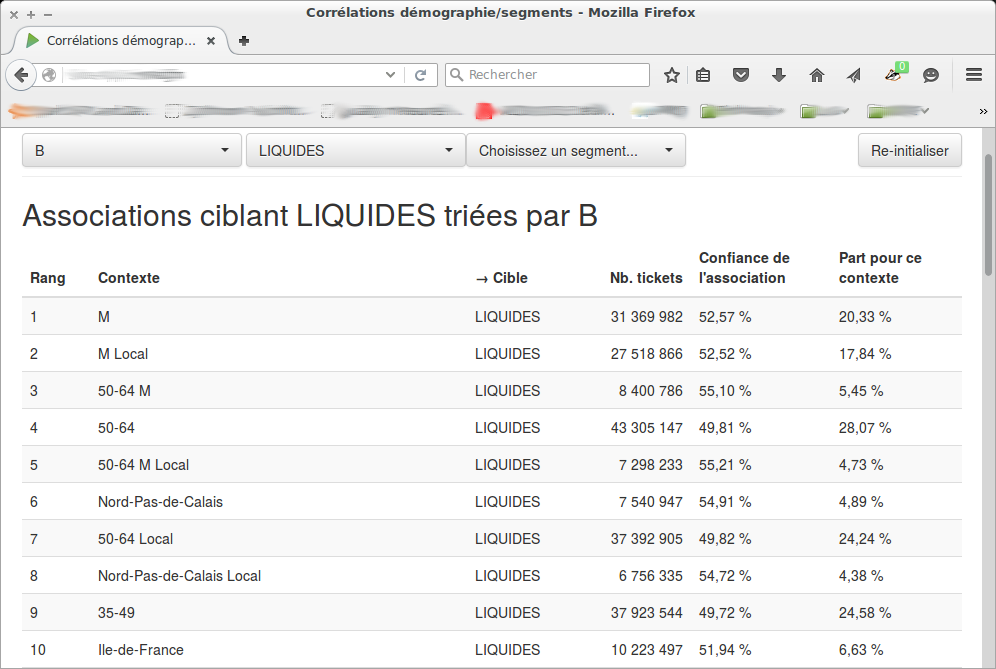
\includegraphics[scale=0.10]{fig/screenshot_exploration.png}};
    \node [number] (dot6) at ($(webapp)+(1.7,1)$) {5};

    %%%
    %%% ARROW: DATABASE to WEBAPP
    %%%
    \draw [big black arrow=0.5] (rules) -- (webapp);

    %%%
    %%% BOUNDING-BOX: EXPLORATION
    %%% id: blueBox
    %%%
	\begin{pgfonlayer}{background}
	  \path (webapp.north west)+(-0.6,0.1) node (boxLTopLeft) {};
	  \path (webapp.south east)+(0.6,-1) node (boxLBottomRight) {};
	  \node [rectangle,fit=(boxLTopLeft) (boxLBottomRight),fill=black!5,
        rounded corners,
	      draw=black!50] (blueBox) {};
	\end{pgfonlayer}

    %%%
    %%% BOUNDING-BOX-LABEL: EXPLORATION
    %%%
    \path (webapp.south) +(0,-0.6) node [font=\large] (boxBL) {{\bf Exploitation} (\capa)};

    %%%
    %%% ARROW: RULES to DATABASE
    %%%
    %\coordinate (magicHinge) at ($(database.south-|rules)+(0,1)$);
    %\path (database.south -| magicHinge)+(0,-1) node[] (pointDatabase) {};
    %\path (rules.north -| magicHinge)+(0,-0.25) node[] (pointRules) {};
    %\path (database.south -| rules)+(0,0.2) node[] (pointDatabase) {};
    %\draw [big black arrow=0.8] ($(rules)+(0,-0.2)$) to node[above,xshift=0.2cm,yshift=0.1cm]{Enrichment with measures} (pointDatabase);
    %\draw[out=270,in=90,big black arrow=0.99] (tickets.south) to node[above,xshift=-0.6cm]{Batch Transfer} (sales.north);



    %%%%%%%%%%%%%%%%%%%%%%%%%%%%%%%%%%%%%%%%%%%%%%%%%%%%%%%%%%%%%%%%%%%%%%
	%%%%%%%%%%%%%%%%%%%%%%%%%%%%%%%%%%%%%%%%%%%%%%%%%%%%%%%%%%%%%%%%%%%%%%
	%%%%%%%%%%%%%%%%%%%%%%%%%% FINISH: PART IV %%%%%%%%%%%%%%%%%%%%%%%%%%%
	%%%%%%%%%%%%%%%%%%%%%%%%%%%%%%%%%%%%%%%%%%%%%%%%%%%%%%%%%%%%%%%%%%%%%%
	%%%%%%%%%%%%%%%%%%%%%%%%%%%%%%%%%%%%%%%%%%%%%%%%%%%%%%%%%%%%%%%%%%%%%%


    %%%
    %%% DECISION BOX
    %%% id: scenarioBox
    %%%
    \node [diamond, shape aspect=1.8, scale=0.8,draw,font=\large] (scenarioBox) at ($(prep.west)+(-4,-2)$)
    {\begin{tabular}{c}\setlength{\tabcolsep}{0pt} Scenario\\+\\Targets\end{tabular}};

    %%%
    %%% ANALYST
    %%% id: browser-c
    %%%
    \begin{pgfonlayer}{foreground}
    	\pic(browser) [
    		draw,
    		fill = gray!30,
    		pic text = {Analyst},
    		scale=0.4
    	] at ($(scenarioBox)+(0,-3)$) {computer};
    \end{pgfonlayer}
    %%%
    %%% ARROW: ANALYST to DECISION BOX
    %%%
    \coordinate (browserBoxRight) at ($(browser-c)$);
    %\coordinate (scenarioBoxLeft) at (scenarioBox|-browserBoxTop);
    \draw [big black arrow=1] (browserBoxRight) -- ($(scenarioBox.south)$);

    \coordinate (choicePivot) at ($(scenarioBox|-curation.south)+(0,-0.3)$);

    \coordinate (choicePivotTranslatedRight) at (choicePivot-|case1);
    \coordinate (choicePivotTranslatedLeft) at (choicePivot-|case3);

    \coordinate (lowprep) at ($(prep.west)+(0,-2)$);

    \draw [big black arrowSmall dashed=0.66] (scenarioBox.east) -- (lowprep);
    %\draw [big black arrowSmall dashed=0.90] (scenarioBox.north) -- (choicePivot) -- (choicePivotTranslatedRight) -- (case1);
    %\draw [big black arrowSmall dashed=0.66] (scenarioBox.north) -- (choicePivot) -- (choicePivotTranslatedLeft) -- (case3);
    %\draw [big black arrowSmall dashed=0.56] (choicePivotTranslated) -- (choicePivotTranslatedLifted) -- (case1);
    %\draw [big black arrowSmall dashed=0.56] (choicePivotTranslated) -- (choicePivotTranslatedSunk) -- (case3);
    %\draw [big black arrowSmall dashed=0.66] (choicePivotTranslated) -- (case2);


    \node [number] (dot3) at ($(scenarioBox)+(2.5,0)$) {3};

    %%%
    %%% ARROW: WEBAPP to ANALYST
    %%%
    %\coordinate (browser-c-shifted) at (browser.south);
    \draw [big black arrow=0.5] (browserBoxRight |- webapp.north) -- (browserBoxRight);

	%%%%%%%%%%%%%%%%%%%%%%%%%%%%%%%%%%%%%%%%%%%%%%%%%%%%%%%%%%%%%%%%%%%%%%
	%%%%%%%%%%%%%%%%%%%%%%%%%%%%%%%%%%%%%%%%%%%%%%%%%%%%%%%%%%%%%%%%%%%%%%
	%%%%%%%%%%%%%%%%%%%%%%%% FINISH: DECISION BOX %%%%%%%%%%%%%%%%%%%%%%%%
	%%%%%%%%%%%%%%%%%%%%%%%%%%%%%%%%%%%%%%%%%%%%%%%%%%%%%%%%%%%%%%%%%%%%%%
	%%%%%%%%%%%%%%%%%%%%%%%%%%%%%%%%%%%%%%%%%%%%%%%%%%%%%%%%%%%%%%%%%%%%%%


\end{tikzpicture}

		\end{minipage}
		\centering
		\caption{\label{fig:archoverview}
			Overview of our complete system
		}
	\end{figure}
\restoregeometry
}



\section{Data provided by \datalyse partners}
\label{sec:pipeline:theirs}


\subsection{Raw data on receipts, customers and products}
\label{sec:model:init}

\begin{figure}
	\centering
	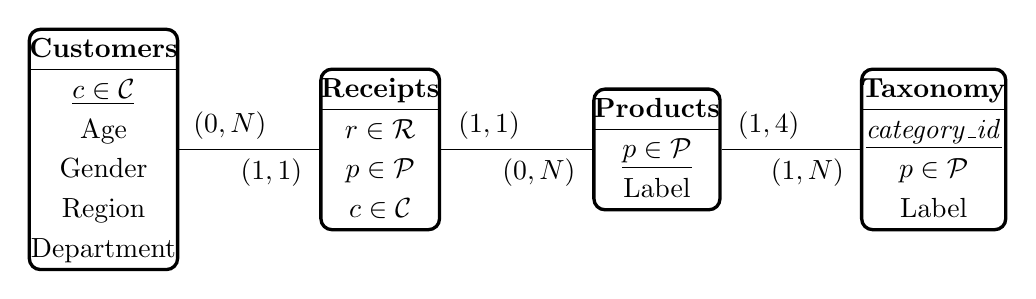
\begin{tikzpicture}
		\tikzset{
  state/.style={
         rectangle,
         rounded corners,
         draw=black, very thick,
         minimum height=2em,
         inner sep=0,
         text centered,
         },
}

    \node[state] (receipts) {
      \begin{tabular}{c}
        \textbf{Receipts}\\
        \hline
        $r \in \cal R$\\
        $p \in \cal P$\\
        $c \in \cal C$
      \end{tabular}
    };

    \node[state,
      left of=receipts,
      node distance=10em,
      anchor=center] (customers)
    {
      \begin{tabular}{c}
        \textbf{Customers}\\
        \hline
        \underline{$c \in \cal C$}\\
        Age\\
        Gender\\
        Region\\
        Department
      \end{tabular}
    };

    \node[state,
      right of=receipts,
      node distance=10em,
      anchor=center] (products)
    {
      \begin{tabular}{c}
        \textbf{Products}\\
        \hline
        \underline{$p \in \cal P$}\\
        Label
      \end{tabular}
    };

    \node[state,
      right of=products,
      node distance=10em,
      anchor=center] (taxonomy)
    {
      \begin{tabular}{c}
        \textbf{Taxonomy}\\
        \hline
        \underline{$\mathit{category\_id}$}\\
        $p \in \cal P$\\
        Label
      \end{tabular}
    };


    \path (customers.east) edge
      node[anchor=west,above,xshift=-0.7em]{$(0,N)$}
      node[anchor=east,below,xshift=0.8em]{$(1,1)$}
      (receipts);

    \path (receipts.east) edge
      node[anchor=west,above,xshift=-1em]{$(1,1)$}
      node[anchor=east,below,xshift=0.8em]{$(0,N)$}
      (products.west);

    \path (products.east) edge
      node[anchor=west,above,xshift=-0.8em]{$(1,4)$}
      node[anchor=east,below,xshift=0.6em]{$(1,N)$}
      (taxonomy.west);

	\end{tikzpicture}

  \caption{\label{fig:schema}
    Entity-relationship diagram of our input data.
    Primary keys are underlined.
  }
\end{figure}

The initial collection is a set of records of the form $\langle r, p, c \rangle$,
where $r$ is a unique receipt identifier (generated at each purchase)
and $p$ is a product purchased by a customer $c$.
When a customer $c$ purchases multiple products at the same time,
several records with the same $r$ and $c$ are generated.
Figure~\ref{fig:schema} summarizes our input's schema.

The set of receipt identifiers, {\mf R}, contains over 290 million entries
spanning 3.5 billion records, generated by a retail chain consisting of \num{1884} stores
over the whole year 2013.
%Multiple receipt identifiers can be associated with the same customer.
The set of customers, {\mf C}, contains over $9$ million identifiers.
Each customer has 4 demographic attributes: {\em age, gender, region} and {\em department}.
The attribute {\em age} takes values in {\em \{<35, 35-49, 50-65, >65\}},
while {\em region} and {\em department} refer to the customer's location
in France's administrative divisions (18 regions, each divided in a few departments).

Demographic attributes are used to form customer segments:
each segment is described by a set of attribute values
interpreted in the usual conjunctive manner.
For example, the segment $\{\mathit{<35},\mathit{Paris}\}$ refers to young Parisian customers.
Given a customer identifier $c \in \cal C$,
the function $\mathit{demo(c)}$ provides its complete record from our {\em Customers} table.
For example, if {\em Mary} is a 48 years old {\em female} from the {\em Calvados} department,
then $\mathit{demo(Mary)} =$ {\em \{35-49, female, Normandie, Calvados\}}.


\begin{figure}
	\centering
	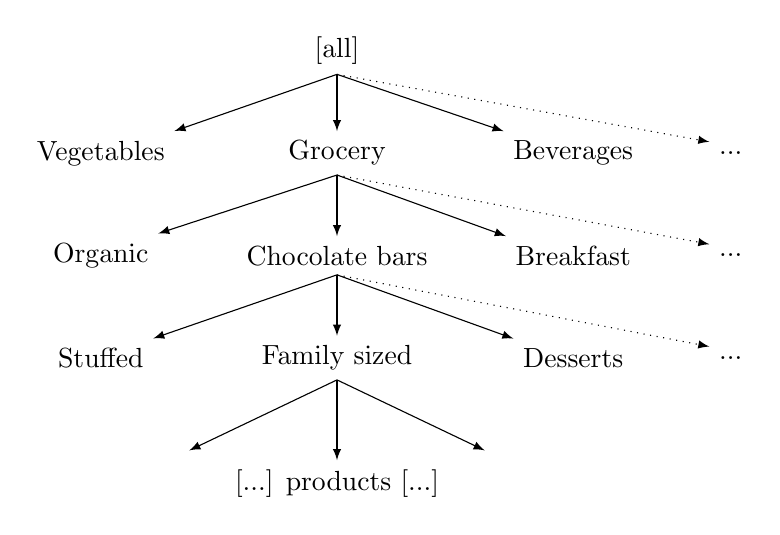
\begin{tikzpicture}[>=latex]
		
\node (root) at (-1,0) {[all]};

\node (A_farleft) at (-4, -1.3) {Vegetables};
\draw [->] (root.south) -- (A_farleft.north east);

\node (A_left) at (-1,-1.3) {Grocery};
\draw [->] (root.south) -- (A_left.north);

\node (A_right) at (2,-1.3) {Beverages};
\draw [->] (root.south) -- (A_right.north west);

\node (A_farright) at (4,-1.3) {...};
\draw [->,dotted] (root.south) -- (A_farright.north west);

\node (B_farleft) at (-4,-2.6) {Organic};
\draw [->] (A_left.south) -- (B_farleft.north east);

\node (B_left) at (-1, -2.6) {Chocolate bars};
\draw [->] (A_left.south) -- (B_left.north);

\node (B_right) at (2, -2.6) {Breakfast};
\draw [->] (A_left.south) -- (B_right.north west);

\node (B_farright) at (4, -2.6) {...};
\draw [->,dotted] (A_left.south) -- (B_farright.north west);

\node (C_farleft) at (-4, -3.9) {Stuffed};
\draw [->] (B_left.south) -- (C_farleft.north east);

\node (C_left) at (-1, -3.9) {Family sized};
\draw [->] (B_left.south) -- (C_left.north);

\node (C_right) at (2, -3.9) {Desserts};
\draw [->] (B_left.south) -- (C_right.north west);

\node (C_farright) at (4, -3.9) {...};
\draw [->, dotted] (B_left.south) -- (C_farright.north west);

\node (D_l) at (-3, -5.2) {};
\draw [->] (C_left.south) -- (D_l.north east);
\node (D) at (-1, -5.5) {[...] products [...] };
\draw [->] (C_left.south) -- (D.north);
\node (D_r) at (1, -5.2) {};
\draw [->] (C_left.south) -- (D_r.north west);

	\end{tikzpicture}
	\caption{\label{fig:taxonomy}
		Extract from our products taxonomy.
		While the 11 top categories are intuitive,
		the \num{19546} others are much more specialized,
		like the ``family-sized chocolate bars'' shown here.
		Lower-level categories also include ``liquid soups for children'', ``men sport socks''
		or ``A4 technical sheets'', for example.
	}
\end{figure}


The set of products {\mf P} contains over \num{200000} entries,
%out of which \num{55786} have been sold more than a thousand times over 2013.
organized in a taxonomy with \num{19557} nodes over 4 levels.
Figure~\ref{fig:taxonomy} shows a sample from our taxonomy.
Products are leaf nodes, and belong to all their ancestor categories.
Given a product $p$, the set of categories it belongs to is denoted as $\mathit{cat(p)}$.
For example, {\em chocolate cream} belongs to the categories
{\em \{Fresh food, Dairy, Ultra fresh, Desserts\}}.


\subsection{Acquisition and storage}
\label{sec:archstore}
%DO WE ONLY KEEP TICKETS WITH A LOYALTY CARDS ? => YES

Each of the \num{1884} stores logs locally all customer
transactions completed during the day.
Whenever a customer checks out, a receipt is generated,
indicating the list of products purchased, their price, as well as potential discounts.
If the customer has and shows a loyalty card, the card identifier is recorded along its receipt.
Otherwise, a unique identifier is generated using a combination of the store identifier and a timestamp.
In our three mining scenarios, we only consider receipts having a genuine card identifier.
Once a day, during each store's closing time, its log is transmitted to the main data center
that centralizes all sales records.

Our experimental platform holds an anonymized copy of these records
(tuples $\langle r, p, c \rangle$ mentioned in Section~\ref{sec:model:init})
and the {\em customers} and {\em taxonomy} tables.
We rely on Hadoop YARN~\cite{yarn} to administrate this dedicated cluster.
All data is stored in an HBase database~\cite{hbase}.
Enrichment and extractions are performed using the Hadoop MapReduce framework~\cite{DeanOSDI04}.

To avoid redundancy and ease data processing,
records are grouped by receipt before being stored in our \textit{sales} table.
Thus, each receipt is a line in the table
and its products list is stored in the \textit{articles} column family.
We leverage HBase's flexibility on columns by recording each product identifier as a column qualifier,
while the corresponding value holds information such as the cardinality or the unit-price.
The row key is written as \textit{storeId-date-customerId-ticketId},
and we set-up an HBase region per store to ensure a good balancing in our cluster.
This allows operations such as extracting the sales of a given store
to be efficiently performed in a single scan,
while selecting a specific time period can also be done by a single key scan.
This data layout is optimized to perform these selections efficiently,
without incurring unnecessary reads.
That allows to store large amounts of data without increasing the cost of analyzing a fixed
number of records.

When registering for loyalty cards,
customers provide demographic information which can be leveraged by marketing analysts
to better understand customer behavior.
Each customer constitutes an entry in the \textit{customers} table,
which records the segments she belongs to as demographic attributes
(for example, {\em \{>65, male, Paris\}}).
After loading the sales records into the database,
we enrich the \textit{sales} table using a MapReduce job.
Each receipt's row is augmented with the user segment by querying the
\textit{customers} table and copying the segment's attributes
in the \textit{meta} column family, as column qualifiers.
Hence, each receipt is assigned a snapshot of the customer's demographic attributes.




\section{Use cases and systems supporting our work}
\label{sec:pipeline:ours}

This section presents how the last steps of the \datalyse workflow are implemented in our use case,
starting from the instanciation of meaningful transactional datasets.
Thus we reach the point in the workflow where our contributions to the project appear:
mining the dataset, and exploring the mining's result.
These two steps are fully detailed in the following chapters;
in this section we only describe how and in which systems they are integrated.

\subsection{Curation: 3 mining scenarios that fit in our itemset mining model}
\label{sec:scenarios}

In order to construct a transactional dataset $\cal D$,
as described in Section~\ref{sec:model:mining},
our raw records $\langle r, p, c \rangle$ can be

\begin{itemize}
	\item joined with the customer's demographic attributes, $\mathit{demo}(c)$;
	\item joined with the products taxonomy,
		to augment each record with the products' categories, $\mathit{cat}(p)$;
	\item then, grouped by any of these attributes.
	We usually group records at least by receipt identifiers.
\end{itemize}

This manuscript follows three mining scenarios designed by experienced analysts
from the marketing studies department of Intermarch\'e.
They are interested in studying two kinds of buying patterns:
those representing associations between customer segments and a product category
(e.g. {\em young people in the north of France consume soda}),
and those associating a set of products to a single product
(e.g. {\em people who purchase pork sausage and mustard also buy dry Riesling}).

In the first scenario, \demoassoc,
the analyst expects rules of the form {\em customer segment} $\rightarrow$ {\em category}.
Such a rule quantifies how customers belonging to the described segment purchase products in the given category.
In that case, ${\cal I}$ is the union of the demographic attributes set and the products categories' set.
We perform the two joins mentioned above, and group records by customer identifier
(additional groupings can be done, as discussed below).

In the two other scenarios, the analyst expects rules of the form {\em set of products} $\rightarrow \{p\}$,
where $p$ is a single product.
$\cal I$ is therefore the set of products.
In the second scenario, \prodassocreceipt, raw records are grouped by receipt identifier $r$.
The resulting transactions are equivalent to the actual receipt given to the customer,
except we ignore multiple purchases of a single product.
In the third scenario, \prodassocclient, records are joined with customer identifiers and grouped by these.
Its goal is to study how products are purchased by customers over time.

The following page gives, for each scenarios,
a few examples of transactions and desired association rules.

\vfill
\pagebreak
\begin{table}[t!]
\centering
\begin{scriptsize}
\def\arraystretch{1.5}
\begin{tabular}{p{0.95\textwidth}}
  MOULIN. MODULE PETIT DEJEUNE, BALAI PVC 60CM SM \\
  BRANDADE MORUE 300G, MOISSON 6 OEUFS, HC240X220+2TO OCEAN, DH 140X190 OCEAN, TT 90X185 OCEAN \\
  CROQUET.ADULTE 10KG \\
  HARICOT VERT EF4/4 440G, BOXER X2 3D FLEX, LIQ. TAPIS MOQUETTE 600ML, MOUCH.ETUIS 15X10, SALADE MELANGE 250G\\
  CAMEMBERT NOIR 250G, KNACKS X20 700 GR, COMTE 6M PORTION 350G, CHEVRE LONG 180G, SALADE MELANGE 250G \\
  CIDRE RGE CELLIER, CIDRE CELLIER 6*75, BUCHE FONDANTE250G, BOURGUIGNON+PDT PERSILLEES 1KG, GALET ROIS POMME 400G, BEURRE DOUX PQ 250G, PUREES AV.OIGN/CIBOULE.375G, BEURRE 1/2 SEL 500G+100G   \\
\end{tabular}
\caption{
  Extract from our \prodassocreceipt dataset (items are separated by commas, brand names removed).
  \prodassocclient is similar, except transactions usually contain ten times more products.
  \label{tab:extracts:products}
}
\end{scriptsize}
\end{table}



\begin{table}[t!]
\centering
\begin{scriptsize}
\def\arraystretch{1.2}
\begin{tabular}{|c|c|c|}
  \hline
  $A \rightarrow B$       & $\mathit{support}(A)$ & $\mathit{support}(A \cup B)$ \\\hline
  LIEGEOIS CHOCO 4X100G $\rightarrow$  CR.DESS.CHOCO 4X115G       & \num{477710}& \num{98693}   \\
  \{P.FEUILLT ROULE, PREP.FRANGIPANE\} $\rightarrow$ SUCRE POUDRE 1/2KG & \num{9743} & \num{522}  \\
  \{ALGUES NORI 17.50G, WASABI 43G, SAUCE SOJA JAP 200ML\} & & \\
                             $\rightarrow$ RIZ SUSHI 450G & \num{212}     & \num{133}   \\
  \hline
\end{tabular}
\caption{
  Example association rules extracted from \prodassocreceipt
  (we search similar rules in \prodassocclient).
  \label{tab:extracts:products:rules}
}
\end{scriptsize}
\end{table}


\begin{table}[t!]
\centering
\begin{scriptsize}
\def\arraystretch{1.5}
\begin{tabular}{p{0.95\textwidth}}
  {\em <35, Male, Auvergne, Allier}, SURGELES, CRUSTACES, BISCUITS FRUITES, BALLADEUR AUDIO,
    PETITE PUERICULTURE, D.P.H., MOUCHOIR \& PAPIERS HYGIENIQUES, ... \\
  {\em <35, Female, Rhône-Alpes, Isère}, FRUITS ET LEGUMES, F/L FRAIS EMBALLE, F/L RAYON REFRIGERE DLC COURTE,
    EPICERIE SALEE, FARINES, FARINE PREPA PAINS, ... \\
  {\em >65, Male, Poitou-Charentes, Vienne}, SAUCISSERIE, SURIMI, BOUL PAT TRAD, VIENNOISERIE TRAD,
    TRAITEUR TRAD, LIQUIDES, APERITIFS SANS ALCOOL, EAUX MINERALES, ...\\
  {\em 50-65,  Female, Franche-Comté, Haute Saône}, D.P.H., MAQUILLAGE, MAQUILLAGE COFFRETS, CREMERIE LS, BEURRE LS, OEUFS, PRODUITS CULTURELS,
    JEUX CONSOLES, FROMAGE TRAD, FROMAGE COUPE, SPECIALITES REGIONALES, ... \\
  {\em  50-65,  Female, Franche-Comté, Haute Saône}, CHARCUTERIE TRAITEUR, CRUDITES, SANDWICH, FOIES GRAS,
    PAIN PAT LS INDUS, PAIN DE MIE ET ASSIMILES, PAINS PRECUITS, ...\\
\end{tabular}
\caption{
  Extract from our \demoassoc dataset, with shortened transactions as customers
  are usually buying products from dozens of categories,
  because each product contributes its 4 containing categories here.
  Demographic attributes are italicized.
%  As described in Section~\ref{sec:model:curation},
%  the actual file stores, for each distinct customer segment,
%  the number of occurrences of each products category.
%  For example, the two last lines of this example are grouped.
  \label{tab:extracts:demo}
}
\end{scriptsize}
\end{table}


\begin{table}[t!]
\centering
\begin{scriptsize}
\def\arraystretch{1.2}
\begin{tabular}{|c|c|c|}
  \hline
  $A \rightarrow B$       & $\mathit{support}(A)$ & $\mathit{support}(A \cup B)$ \\\hline
  {\em Alsace} $\rightarrow$ PAINS DE CAMPAGNE & \num{2843532} & \num{28889}  \\
  {\em 35-49, Female} $\rightarrow$  PRODUITS SOLAIRES  & \num{49677175}& \num{196612}   \\
  {\em >65, Nord, Nord-Pas-de-Calais} $\rightarrow$ CHAMPAGNES MILLESIMES  & \num{2957290}     & \num{1187}   \\
  \hline
\end{tabular}
\caption{
  Example association rules extracted from \demoassoc.
  \label{tab:extracts:demo:rules}
}
\end{scriptsize}
\end{table}

\pagebreak
\clearpage


For the 3 mining scenarios,
the corresponding dataset is created using MapReduce jobs on the \textit{sales} table,
and stored on HDFS as a text file with one line per transaction.

In the \prodassocreceipt case,
the set of product identifiers, from each line of our \textit{sales} table, generates one transaction.
As records are already grouped by receipt, this is a \verb|map|-only job,
resulting in a 23.4GB file.

For \prodassocclient, the products bought by each customer are grouped using a \verb|reduce| operation,
where the customer identifier is the key.
For each customer, the resulting products set is outputted as a transaction,
yielding a 13.3GB file.

Generating transactions for the \demoassoc scenario also requires a single MapReduce job,
but is less straightforward.
In this case the analyst searches for rules of the form {\em customer segment} $\rightarrow$ {\em category},
hence we need transactions of the form {\em \{category, demographic attributes [\ldots]\}}.
But writing such transactions would generate many duplicates,
because thousands of customers are usually represented by a single segment ({\em ie.} a given attributes set).
Moreover, in this case we search for associations leading to a {\em single} category.
Categories are never combined in an itemset,
so we can further group the transactions in order to write a line per customer segment.
Each line stores how many times customers from this segment bought a product from each available category.

Therefore the dataset curation for \demoassoc starts with a \verb|map|-side join.
All mappers load the products taxonomy in memory (through the distributed cache) and,
for each product in each row,
generate as many $\langle \mathit{segment}, \mathit{category} \rangle$ records as
the product has categories in the taxonomy.
Customer segments are directly available in the \textit{meta} column family,
thanks to the enrichment phase.
Then, for each segment ({\em ie.} for each distinct demographic attributes set),
the \verb|reduce| phase can count how many times each category has been purchased.
The counters are outputted in a single record, along their corresponding segment.
This double grouping gives a very compact representation of the receipts:
for the whole year 2013, the resulting file is only 39MB large.

Grouping identical transactions is surprisingly inefficient for the receipts datasets.
Only \num{35394} transactions (0.4\%) can be merged in \prodassocclient,
and \num{26232544} (9\%) in  \prodassocreceipt -
not enough to compensate the cost of storing an additional weight with each transaction,
especially as only short transactions are merged.
This suggests that a products set can be enough to identify a customer with a decent accuracy.
But in this work we leave aside privacy considerations (access to this data is restricted)
and send datasets to the mining programs.



\subsection{Experimental and production platforms}
\label{sec:datalyse:prod}

The mining step is the execution of one of the two algorithms we implemented, \jlcm and \toppi,
which are respectively presented in Section~\ref{sec:jlcm} and Chapter~\ref{chap:toppi}.
Thorough our experiments they may run on two hardware settings,
which will be referred to as \textit{server} and \textit{cluster}.

Hadoop programs are deployed on the \textit{cluster} configuration,
which consists of up to 65 machines running Hadoop 1.2.1 (without speculative execution),
one of them acting as the master node.
Each machine contains 2 Intel Xeon E5520 4-cores CPUs and 24 GB of RAM.
We use the default configuration, except for resource allocation.
The number of tasks per machine and the memory allocated to each is detailed for each experiment.

Multi-threaded implementations run on the \textit{server} configuration:
a single machine containing 128GB of RAM and 2 Intel Xeon E5-2650 8-cores CPUs with Hyper Threading,
allowing up to 32 threads in parallel.

%We presented the logical and physical architectures of the {\em experimental} platform
%which backed the present effort.
It is worth mentioning that the production architecture, set up by our industrial partners in \datalyse,
is logically equivalent but deployed differently.
The only common point is the curation platform.
The production platform is a YARN cluster made of 4 worker nodes.
Each one is a virtual machine which has been assigned 32GB of RAM and
4 cores out of the 8 of an Intel Xeon E5-2650L CPU.
In production, this YARN cluster is also the analytics platform, running the mining step.
This sets the bar for our resource requirements:
on this cluster, our algorithms should be able to run the mining step of our 3 scenarios.

%As we will see, we meet these requirements:
%for some datasets even the author's laptop is sufficient.



\subsection{Result exploration and exploitation}

Finally, the user needs a tool to explore, filter and sort the discovered association rules.
The target audience of this tool is not only computer scientists
or data analysts from Intermarch\'e, but also marketing experts.
Hence an interactive and highly intuitive tool is required at this step.
%This is also crucial for \capa's user study (presented in Chapter~\ref{chap:capa}).

We therefore developed a Web application which present results stored in a PostgreSQL database~\cite{postgres}.
The amount of association rules we generate (usually in the millions)
is easily handled by a classic setup on a dedicated virtual machine.


\vfill
\pagebreak

\section{Datasets summary: common characteristics}
\label{sec:model:conc}

\begin{table}[t!]
\centering
\begin{tabular}{|c|c|c|c|c|}
\hline
{\bf Dataset}     & {\bf \#Transactions} & {\bf \#Items} & {\bf File size} & {\bf Average trans-} \\
                  &                      &                &                & {\bf -action length} \\ \hline
{\em LastFM}      & \num{1218831}   & \num{1206195}&  277 MB  & 47  \\
{\em WebDocs}     & \num{1692082}   & \num{5267656}&  1.4 GB  & 177  \\
\demoassoc        & \num{2398}      & \num{241921} &  39 MB   & 1617 \\
\prodassocreceipt & \num{290734163} & \num{222228} &  23.4 GB & 12 \\
\prodassocclient  & \num{9267961}   & \num{222228} & 13.3 GB  & 213 \\
\hline
\end{tabular}
\caption{Our datasets' cardinalities.
\demoassoc is actually a compressed representation of our transactions of interest
(see Section~\ref{sec:scenarios}, p.\pageref{sec:scenarios});
during the mining, the algorithm interprete these as transactions of at most 5 items (see Section~\ref{sec:capa:mining}, p.\pageref{sec:capa:mining}).
\label{tab:datasets}
}
\end{table}


In order to validate the performance of our mining algorithms beyond our industrial setting,
we also run experiments on Web data.
Although our transactional datasets represent very different entities,
they share some properties that raise new challenges for existing closed itemsets (CIS) mining algorithms.
Before developing and answering the different challenges in the following chapters,
we present our 5 datasets of choice and highlight these common properties.
Table~\ref{tab:datasets} summarizes our datasets' details.

Our first two are Web datasets. % which carry different semantics:
The first one {\em LastFM}, represents user activity on a music recommendation website.
We crawled 1.2 million public profile pages,
each resulting in a transaction containing the 50 favorite artists of a user.
Hence in this dataset we mine associations between artists.
The other, {\em WebDocs}, is a dataset frequently used in the itemset mining community~\cite{LuccheseFIMI04}.
 Each transaction contains the words used on a Web page.

% \textit{LastFM} is .
% We crawled 1.2 million public profile pages, resulting in a 277MB input file.
% Each transaction contains the 50 favorite artists of a user,
% hence we mine associations between artists.
% In this dataset an association $\{a,b\}\rightarrow\{c,d\}$ represents how many
% listeners of artists $a$ and $b$ are also listeners of $c$ and $d$.
% We found 1.2 million different artists.
%
% \textit{WebDocs} is a dataset frequently used in the itemset mining community~\cite{LuccheseFIMI04}.
% Each transaction contains the words used in a Web page,
% thus $\{a,b\}\rightarrow\{c,d\}$ represents how many pages containing the words $a$ and $b$ also contain $c$ and $d$.
% There are 1.7 million transactions and 5.2 million different items,
% in a 1.4GB file.

Our three other datasets represent supermarket data,
from which we want to extract insights on consumer behavior.
As detailed in Section~\ref{sec:scenarios},
these studies are formalized as three mining scenarios:
\prodassocreceipt, \prodassocclient and \demoassoc.
The first step of the \datalyse workflow is the transformation of this data into a transactional dataset;
depending on the scenario, transactions may carry different semantics.
In \prodassocreceipt and \prodassocclient a transaction is a set of products chosen by a single customer,
in a single purchase or over the year 2013, respectively.
Hence transactions are longer in \prodassocclient.
In \demoassoc a transaction represents product categories chosen by a customer in a demographic segment.

% In these three scenarios, the transformation in transactionnal datasets allows us to use itemset mining algorithms,
% which are a natural choice to search the desired associations.
% Indeed the resulting itemsets can be converted to association rules as
% $\mathit{bread \rightarrow \{butter, jam\}}$ or $\{\mathit{ <35, Paris}\}\rightarrow \{\mathit{Sodas}\}$.
%

Using a generic model for closed itemsets mining (detailed in Section~\ref{sec:model:mining}, p.\pageref{sec:model:mining})
allows us to experiment with various data.
%The datasets {\em LastFM} and {\em WebDocs} further validate our algorithms'
%performance and show their applicability to other domains.
Whether originating from our industrial partner, from the itemset mining community or from the Internet,
our transactional datasets are representative data
that motivates our adaptations of itemset mining:
millions of short transactions over a few hundred thousands items (or more), with a long tail distribution.
This is illustrated in Figure~\ref{fig:itemFreqDist}
where we can observe that the majority of items occur in less than a hundred transactions.

\begin{figure}
	\centering
	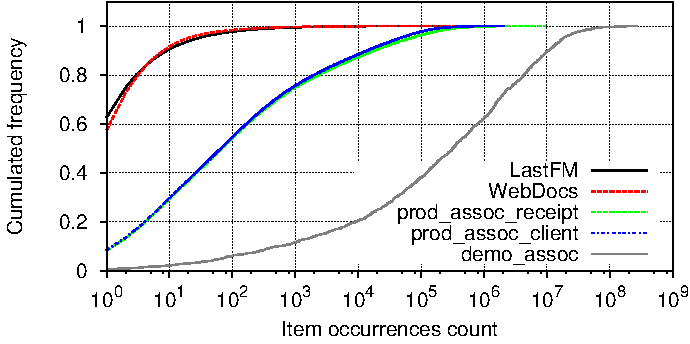
\includegraphics{fig/itemFreqCumulativeDist/itemFreqCumulativeDistributions.pdf}
	\caption{\label{fig:itemFreqDist}
		Cumulative distribution of items' supports in our datasets.
		They form three groups, from top to bottom:
			Web datasets ({\em LastFM} and {\em WebDocs}), have the most pronounced long tail distribution.
			Receipts sets also follow this trend.
			The last one, \demoassoc, is an outlier here because it's mixing hierarchical items
			({\em e.g.} narrow or wide categories).
		}
\end{figure}

This is even more striking for the two Web datasets, {\em LastFM} and {\em WebDocs},
as 90\% of their items occur in at most 10 transactions.
For example, in {\em LastFM} this means that 90\% of artists have 10 listeners or less.
In {\em WebDocs}, 90\% of words appear in 10 documents or less.
These are typical examples of a ``long tail'' distribution~\cite{GoelWSDM10}.
The sparsity of market baskets is more pronounced on non-singleton itemsets:
the support of a pair of items is usually two orders of magnitude lower than
the support of each item alone.
\demoassoc does not show this long-tail distribution,
and its compact representation does not raise any computational challenge.
However the variety of its items makes it relevant to our work on exploring association rules.
The 5 datasets also have in common a low itemset density:
items are spread irregularly in the dataset, and rarely combine with each other.

Each dataset carries its own patterns semantics,
but the techniques presented in the following chapters can be applied to any of them.
% This work started by a re-implementation of PLCM~\cite{NegrevergneHPCS10}.
% The result, \jlcm, is a fast closed itemset miner.
% Choosing the Java language eases the integration in our system
% and provides a simple API for the implementation of constraints on the enumerated itemsets.

% Preliminary experiments with our industrial partners from the \datalyse project showed two limitations.
% The first is that frequent items and itemsets are a minority in our datasets.
% Hence most of the available items are filtered out of the results.
% The second is the quantity of results ---
% even when selecting, for example, those containing a single item of interest.
% We propose, in the following chapters,
% two solutions to overcome each limitation.
